\documentclass[a4paper, 12pt]{article}%тип документа

%отступы
\usepackage[left=1.5cm,right=1cm,top=2cm,bottom=3cm,bindingoffset=0cm]{geometry}
\setlength{\parindent}{5ex}

%Русский язык
\usepackage[T2A]{fontenc} %кодировка
\usepackage[utf8]{inputenc} %кодировка исходного кода
\usepackage[english,russian]{babel} %локализация и переносы

%Вставка картинок
\usepackage{graphicx}
\graphicspath{{pictures/}}
\DeclareGraphicsExtensions{.pdf,.png,.jpg,.bmp,}
\usepackage{wrapfig}

%Графики
\usepackage{pgfplots}
\pgfplotsset{compat=1.9}

%Математика
\usepackage{amsmath, amsfonts, amssymb, amsthm, mathtools}

%Таблицы
\usepackage{longtable} 
\usepackage{float}

%Римские цифры
\newcommand{\RomanNumeralCaps}[1]{\uppercase\expandafter{\romannumeral#1}}

\usepackage{multirow}


\begin{document}
	\begin{titlepage}
		\begin{center}
			\textsc{Федеральное государственное автономное образовательное учреждение высшего образования«Московский физико-технический институт (национальный исследовательский университет)»\\[5mm]
			}
			
			\vfill
			
			\textbf{Лабораторная работа: \\[3mm]
				Интерферометр Тваймана-Грина
				\\[50mm]
			}
			
		\end{center}
		
		\hfill
		\begin{minipage}{.5\textwidth}
			Выполнил студент:\\[2mm]
			Сериков Василий Романович\\[2mm]
			Группа: Б03-102\\[5mm]
			
		\end{minipage}
		\vfill
		\begin{center}
			Москва, 2024 г.
		\end{center}
		
	\end{titlepage}
	
	\newpage
	\textbf{Цель работы: }\\
	
	Собрать интерферометр  Тваймана-Грина и исследовать различные виды аберраций с его помощью.\\ 
	
	\textbf{Теоретические сведения: }\\
	
	\begin{figure}[H]
		\centering
		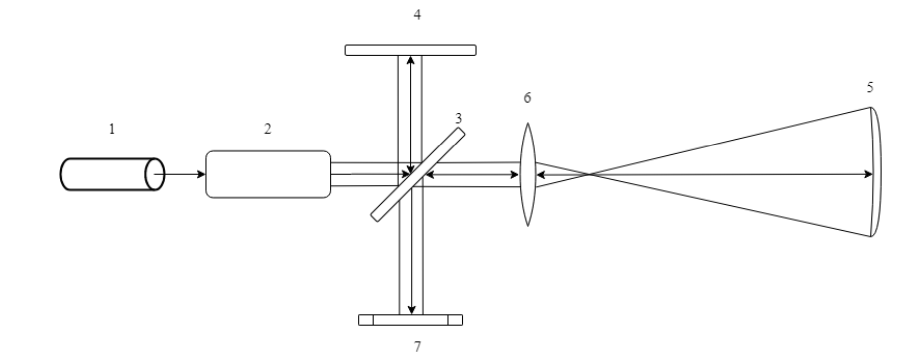
\includegraphics[width=0.9\linewidth]{ust.png}
		\caption{Интерферометр Тваймана-Грина}
	\end{figure}
	
	В качестве источника когерентного света используется лазер 1 (например,
	гелий-неоновый с длиной волны 632,8 нм). Лазерный луч падает на расширитель 2, создающий параллельный пучок. Пучок проходит через светоделитель
	3, разветвляясь на два плеча. В одном плече установлено эталонное зеркало 4,
	формирующее опорный волновой фронт. Во втором плече находится исследуемый элемент 5 — зеркало или линза с плоским зеркалом. При необходимости,
	в это плечо устанавливается дополнительный оптический элемент 6 для изменения геометрии волнового фронта: объектив для формирования сферического
	пучка или нуль-корректор для контроля асферических поверхностей. Оба пучка по возвращению попадают на плоскость наблюдения 7. Как правило, в плоскости наблюдения находится фотоприемник, который измеряет распределение
	интенсивности полученной интерференционной картины.\\
	
	\textbf{Виды аберраций:} \\
	
	\textbf{Дефокусировка} – аберрация с осевой симметрией:
	$$W(\rho) = W_{20}(2\rho^2 - 1)$$
	Ее суть - смещение плоскости изображения вдоль оптической оси, из-за чего
	весь пучок фокусируется ближе или дальше от идеального положения.\\
	
	\textbf{Кома} – вытягивание точки фокусировки в "хвост". Формулы комы 3-го
	порядка:
	$$ W(\rho, \phi) = W^1_{3}(3\rho^3 - 2\rho)\cos\phi + W^{-1}_{3}(3\rho^3 - 2\rho)\sin\phi $$
	
	\textbf{Астигматизм} – искривление фокальной плоскости, плоскость наилучшего
	изображения выгибается "седлом". Формулы астигматизма 3-го порядка:
	$$W(\rho, \phi) = W^2_2 \rho^2 \cos(2\phi) + W^{-2}_2 \rho^2 \sin(2\phi) $$
	
	\newpage
	\textbf{Результаты эксперимента: }\\
	
	\begin{enumerate}
		\item Полученная поверхность без вкручивания винтов:
		
		\begin{figure}[H]
			\centering
			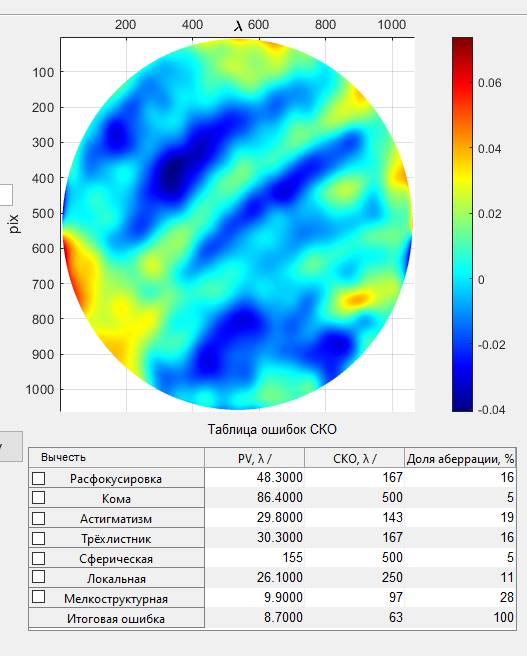
\includegraphics[width=0.9\linewidth]{wo.png}
			\caption{Результат для положения зеркала без давления}
		\end{figure}
		
		\item Поверхность при вкручивании винта в центр оправки на 180$^\circ$ после касания зеркала:

		\begin{figure}[H]
			\centering
			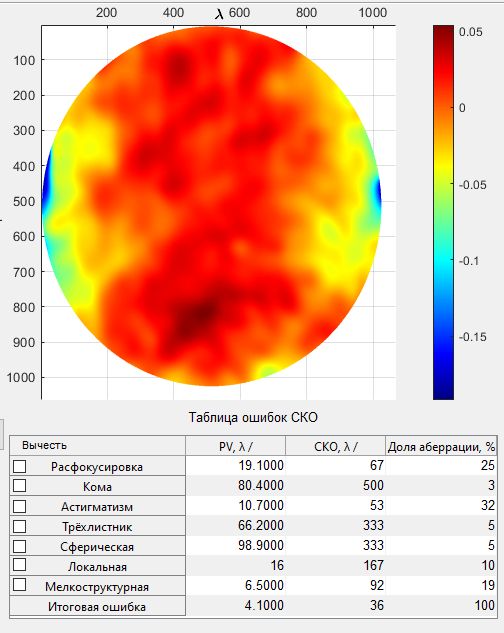
\includegraphics[width=0.9\linewidth]{180.png}
			\caption{Результат для положения зеркала с винтом по центру вкрученном на 180$^\circ$}
		\end{figure}
		\newpage
		\item Поверхность после вкручивания двух винтов по диаметру и картина интерференции:
		
		\begin{figure}[H]
			\centering
			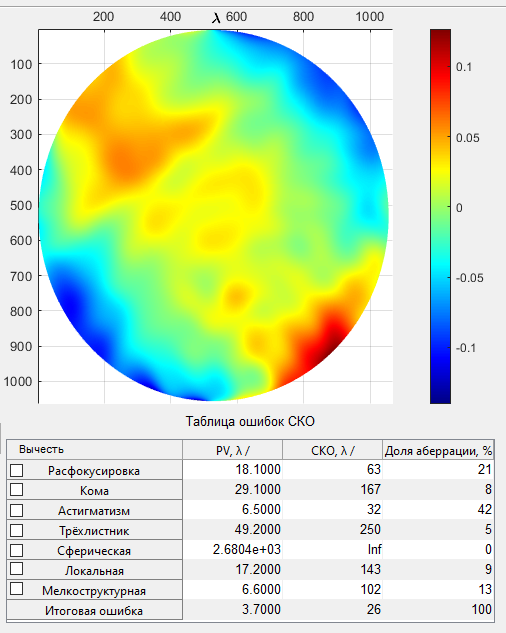
\includegraphics[width=0.9\linewidth]{2ex.png}
			\caption{Поверхность зеркала с двумя винтами по диаметру}
		\end{figure}
		
		\begin{figure}[H]
			\centering
			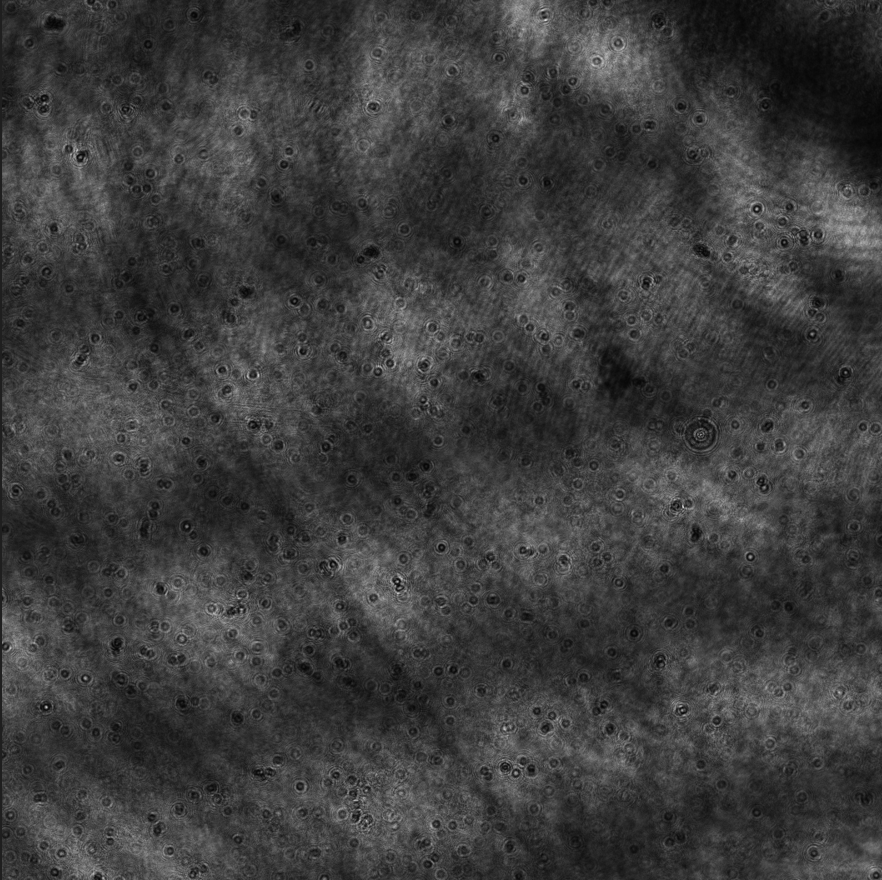
\includegraphics[width=0.9\linewidth]{2ex-lines}
			\caption{Результат интерференции для положения зеркала с двумя винтами по диаметру}
		\end{figure}
		
		\newpage
		
		\item Поверхность после вкручивания винта в край оправки и картина интерференции:
		
		\begin{figure}[H]
			\centering
			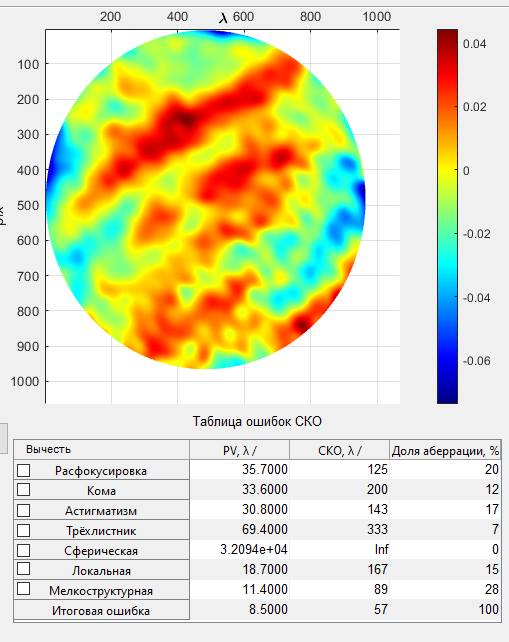
\includegraphics[width=0.9\linewidth]{3ex.png}
			\caption{Поверхность зеркала с винтом на краю оправки}
		\end{figure}
		
		\begin{figure}[H]
			\centering
			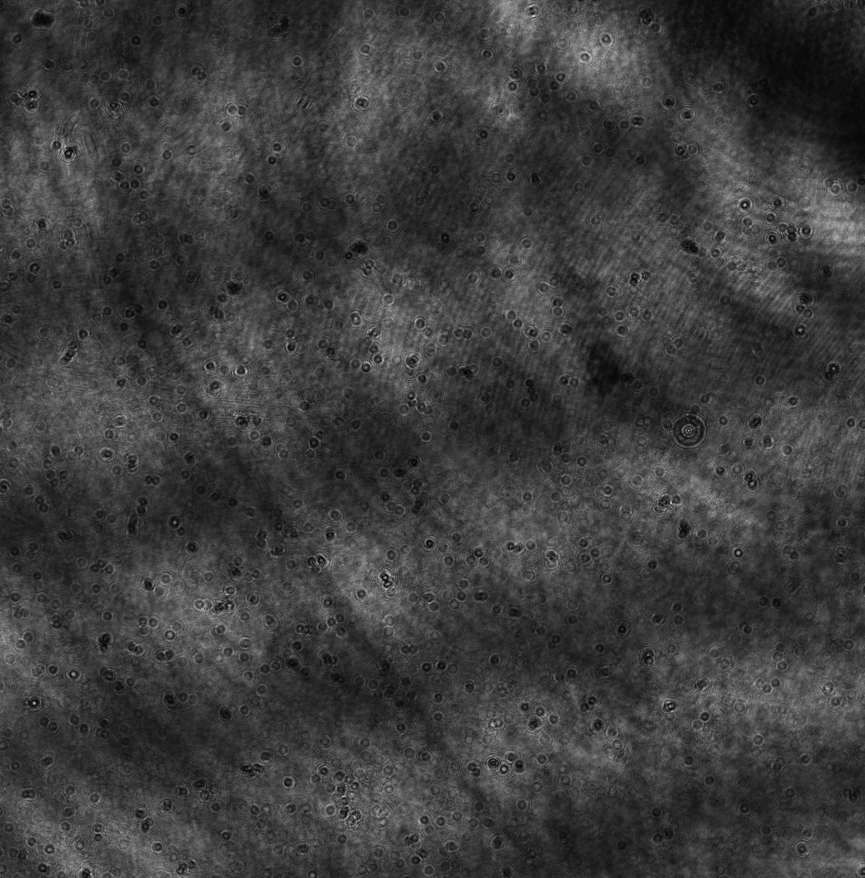
\includegraphics[width=0.9\linewidth]{3ex-lines}
			\caption{Результат интерференции для положения зеркала с винтом на краю оправки}
		\end{figure}
		
	\end{enumerate}
	
	
	\textbf{Обсуждение результатов: }\\
	
	В ходе работы мы хотели получить три вида аберраций: расфокусировка, астигматизм и кома . Но по результатам обработки картин интерференции получили следующие аберрации: астигматизм, астигматизм, мелкоструктурная соответственно. Такие результаты можно списать на не удачное крепление зеркала в оправке, так как зеркало по ходу вкручивания винта может двигаться, тем самым меняя свое положение и нарушая условия эксперимента. 
	
\end{document}